\section{Ergebnisse}

Mit der Anwendung des Programms 





Einleitende Zusammenfassung etc.
\subsection{Auswertung}
%Alle Ergebnisse werden hinsichtlich der Zielsetzung (Anfangshypothesen) bewertet



Ist es möglich mit dem Programm Arnika zu erkennen? 




Begründetes und differenziertes ja: Beispielbilder der verschiedenen Flüghöhen, jeweils Original, Segmentierung, Umrandung




Ist es möglich Arnika zu quantifizieren? Ja schon aber nicht genau genug. Schwierig, siehe Probleme. 
Ist es möglich Arnika zu differenzieren von anderen Blumen? teilweise ja (in den Testbildern ja,1. durch die farbe, 2. da die gewählte Methode zum Ausschluss kleinerer Blüten selber Farbe funktioniert. Bei anderen Blumen, müssen ökologische und geographische Faktoren mitberücksichtigt werden, oder ein anderer Ansatz wie in Literatur -> NN gewählt werden)


%Alle Ergebnisse werden mit relevanter Literatur verglichen und bewertet
NN Beispiel(e) aus der DBU Antrag
weitere?





\subsection{Schwierigkeiten}
\subsubsection{Problem: Kreise um zusammenhängende Blumen}

Bei der Visualisierung der Blumen durch Umrandung, werden vom Programm mehrere Blumen, die zusammenhängen oder überlappen nur mit einem großen Kreis erfasst.

Bei einer Gruppe von Blüten, die überlappen, wird ein zusammenhängende Fläche (ConnectedComponents) bei der gelben Segmentierung heraus gefiltert. Möchte man die Blumen mit Kreisen visualisieren wird der Geometrischer Schwerpunkt der Connected Components (CC) als Mittelpunkt des Kreises gewählt. Als Radius wurde die Höhe oder Breite des CC gewählt, je nachdem welche geringer ist. Hängen nun aber mehrerer Blüten zusammen kann nur ein Kreis mit den Mittelpunkt des gesamten CC gezeichnet werden (Siehe Abbildung~\ref{fig:Kreis}, S. \pageref{fig:Kreis}).
 
\begin{figure}[htb]
 \centering
 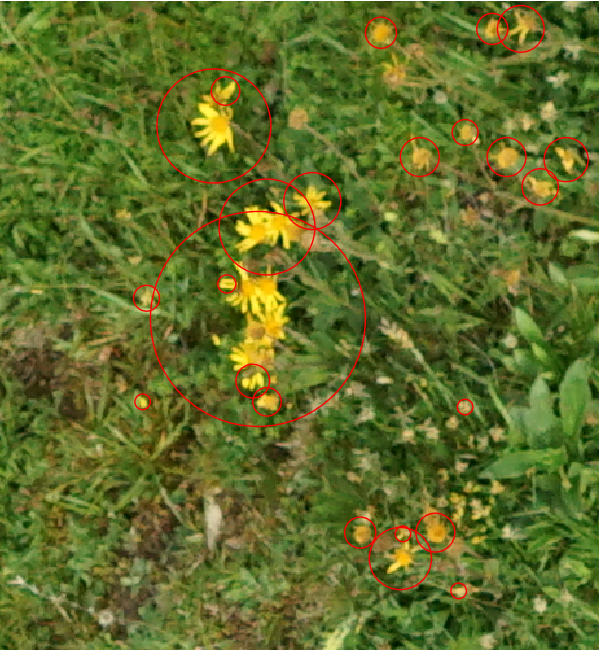
\includegraphics[width=0.4\textwidth,angle=0]{abb/ergebnisse/probleme/bigblob}
 \caption{Ein großer Kreis um zusammenhängende Blumen}
\label{fig:Kreis}
\end{figure}

\paragraph{Lösungsansatz:}
Anstatt einfach den Bildschwerpunkt, der von der Statistik der ConnectedComponents Funktion von OpenCV geliefert wird, wurde versucht die großen CC in ihrem Seitenverhältnis von Höhe zu Breite bzw. Breite zu Höhe zu teilen und mehrere Mittelpunkte anzulegen. 

Idee: center der Kreise bei 1:2, 1:3, 1:4 und 1:5 Verhältnis von Höhe /Breite bzw. Breite zu Höhe verschieben und duplizieren,


\begin{figure}[htb]
 \centering
 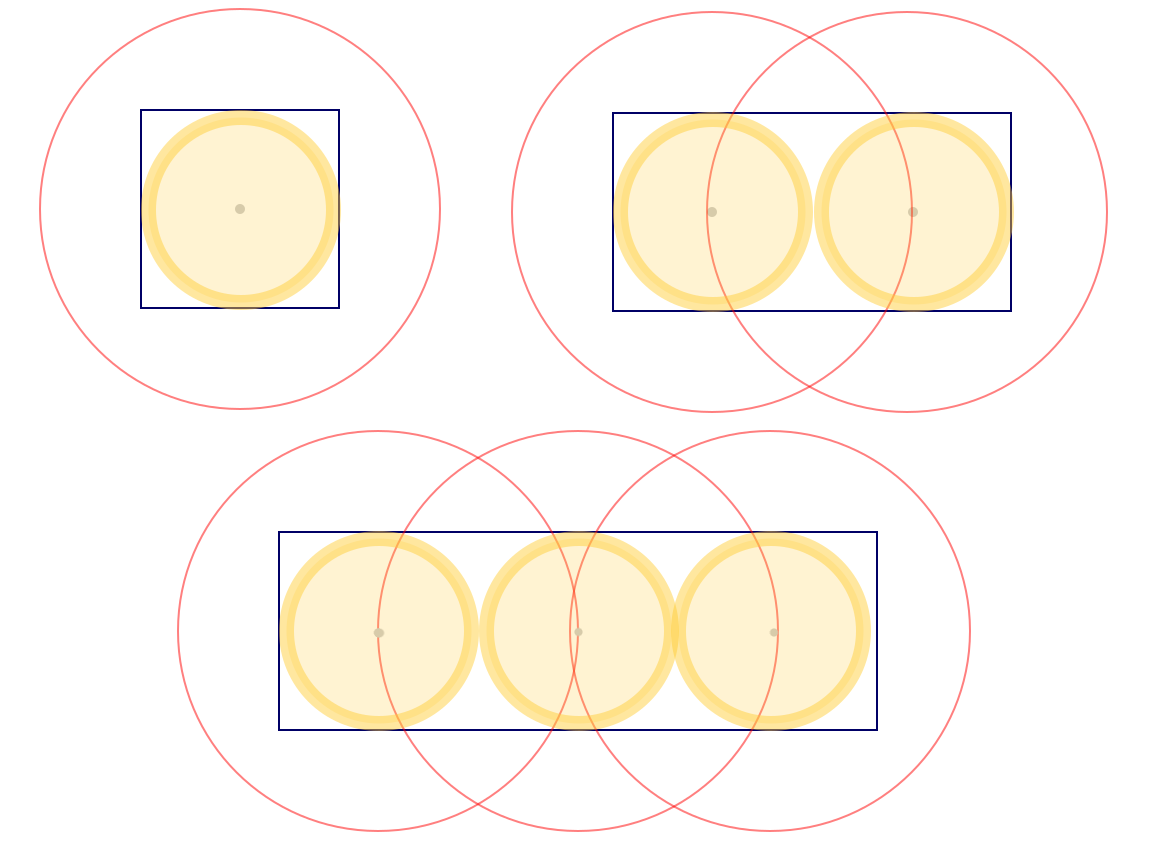
\includegraphics[width=0.5\textwidth,angle=0]{abb/ergebnisse/probleme/seitenverhaeltnis}
 \caption{Schematische Darstellung verschiedener Seitenverhätnisse}
\label{fig:Schema}
\end{figure}


Problem dabei: Wenn eine einzelne Blume aber nicht frontal sondern eher seitlich aufgenommen wurde, hat sie auch dieses Seitenverhältnis und wird auch doppelt gezählt.

\begin{figure}[htb]
 \centering
 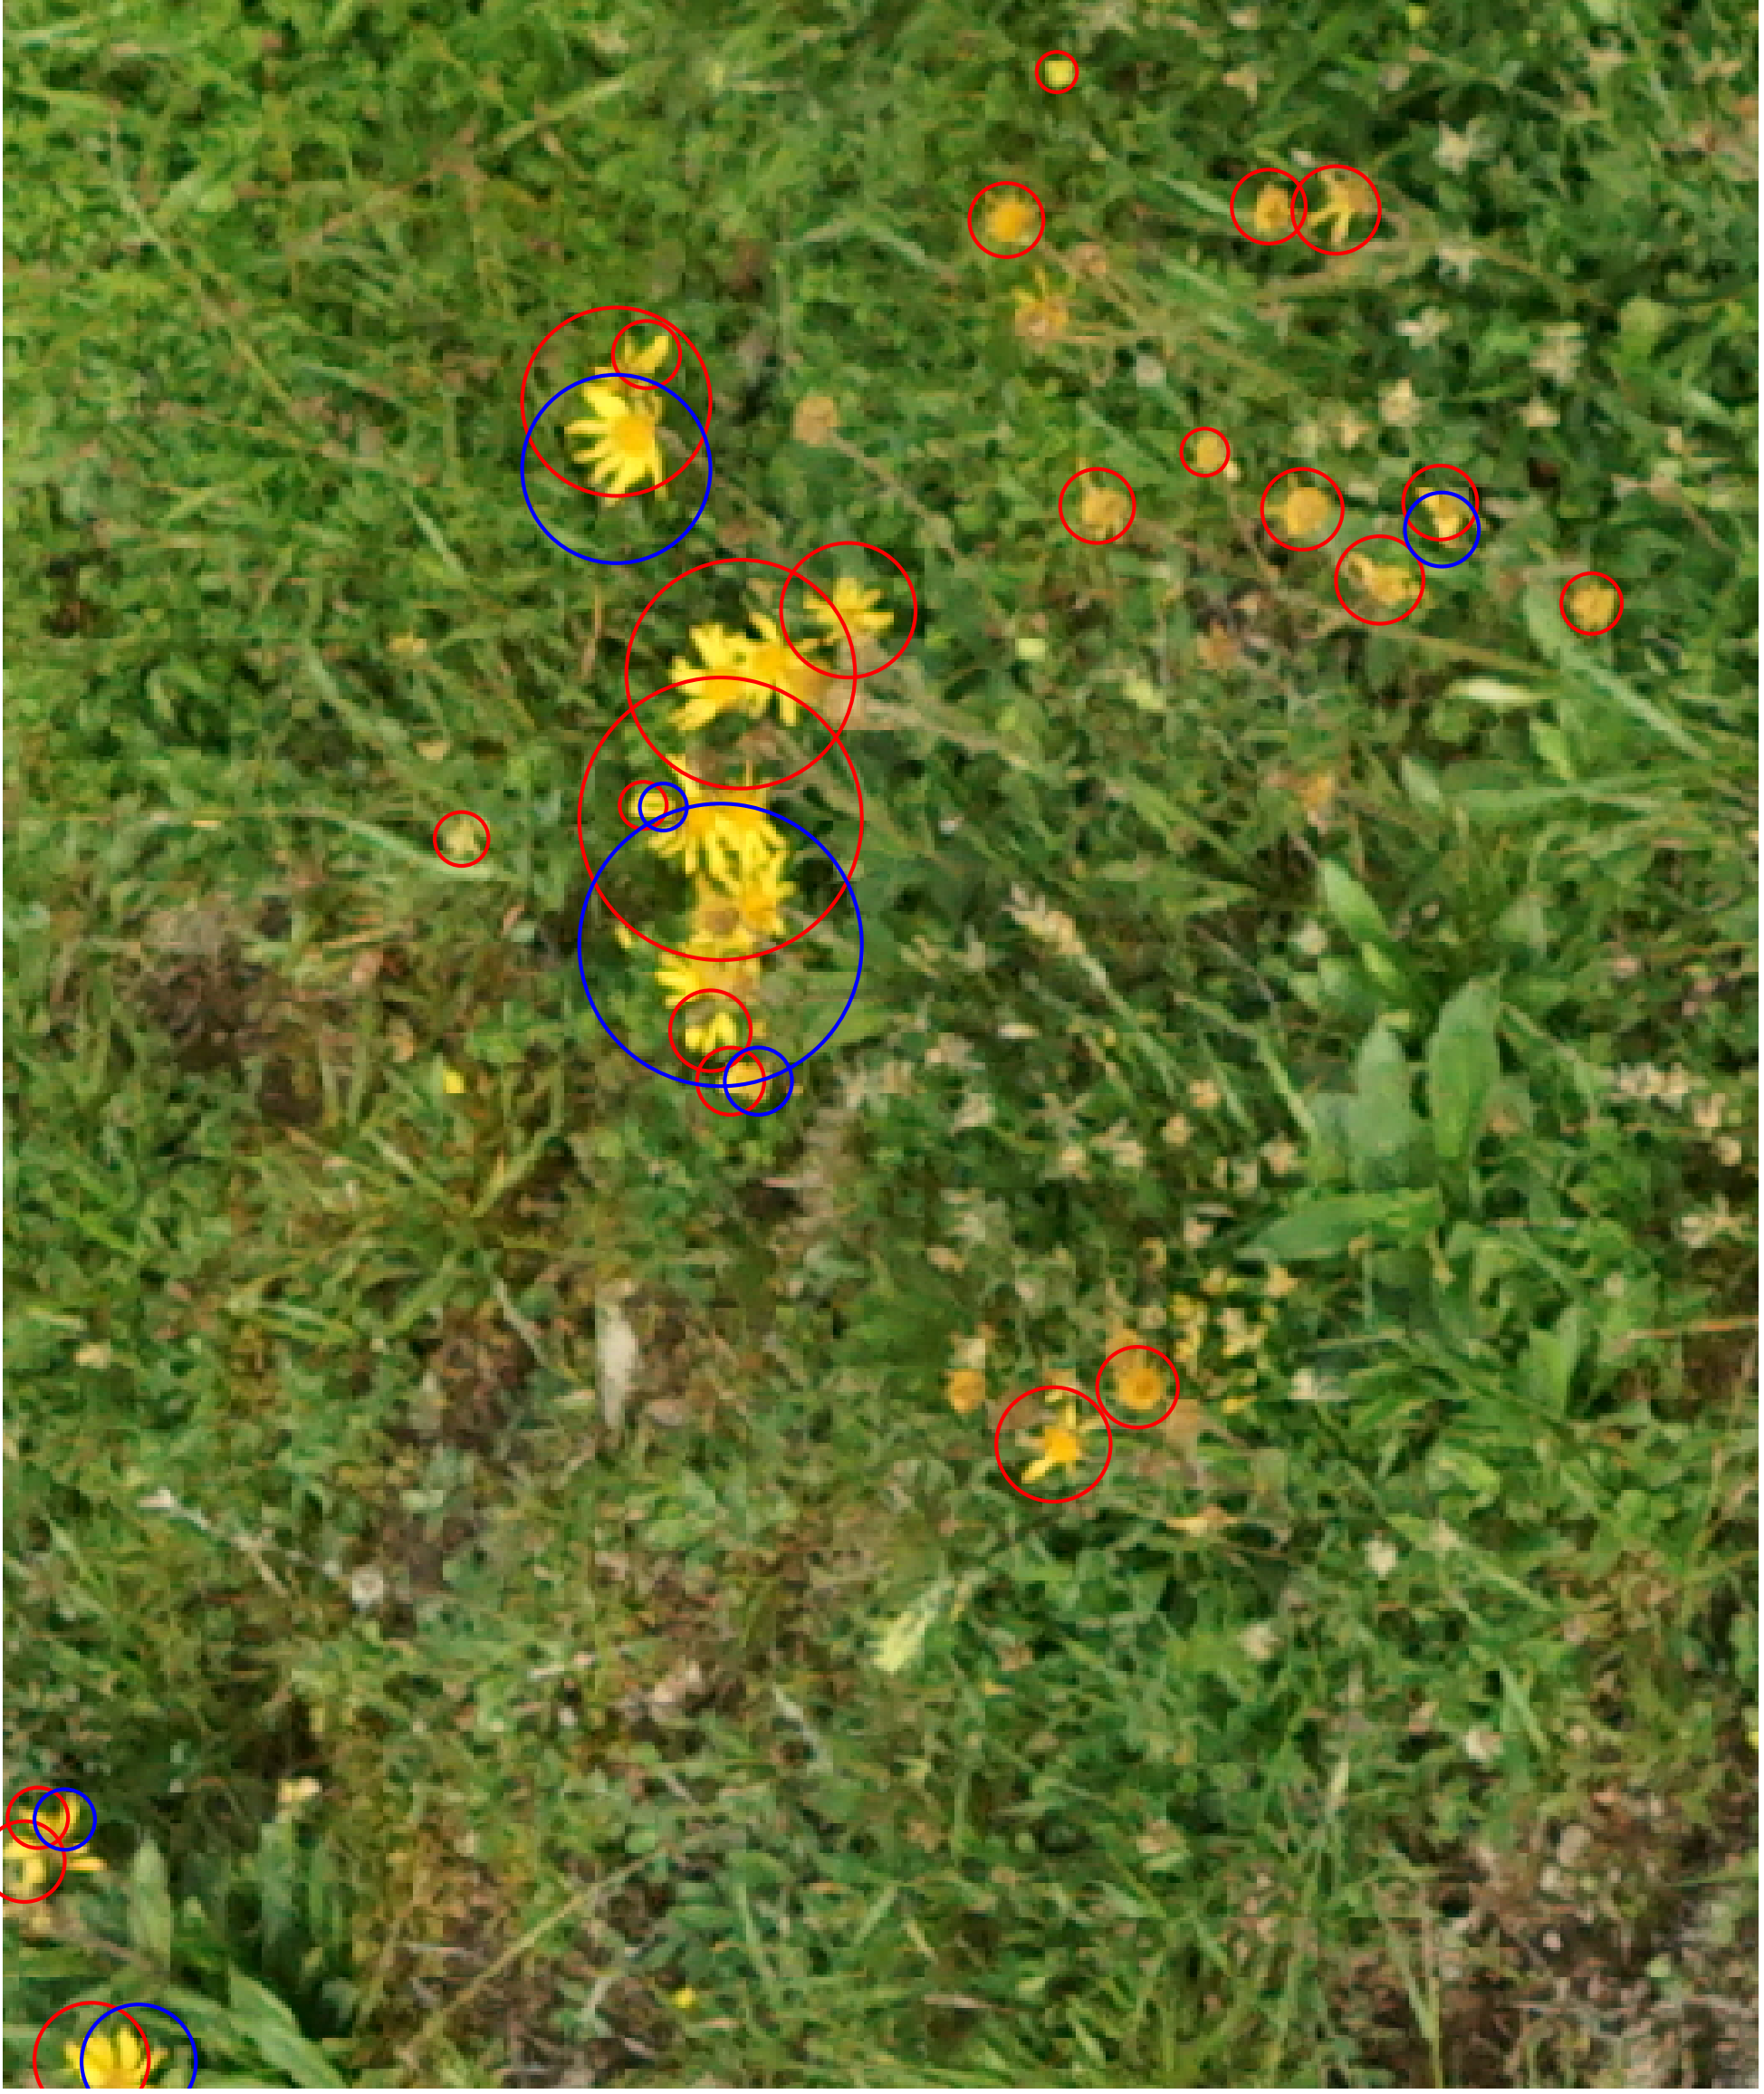
\includegraphics[width=0.4\textwidth,angle=0]{abb/ergebnisse/probleme/circles}
 \caption{Kreise bei nicht proportionalen CC hinzugefügt (blau)}
\label{fig:Kreis-blau}
\end{figure}

Also müsste man das Seitenverhältnis mit der Größe der CC kombinieren. Also die Analyse des Seitenverhältnisses nur bei einer bestimmten Größe beginnen. 
also nicht nur max size, sondern if size > maxsize: die center hinzufügen?

% \blindtext
% \lstset{language=python}
% \begin{lstlisting}[frame=htrbl, caption={Das Listing zeigt Python Quellcode}, label={lst:result2}]
% number, output, stats, centroids = cv2.connectedComponentsWithStats(test.blob[:, :, 0], connectivity=8)
%
% width = stats[1:,2]
% height = stats[1:,3]
% sizes = stats[1:,4]
% number = number - 1
% lowsize = np.mean(sizes)*2
%
% center = np.array((centroids[1:, 0].astype(int), centroids[1:, 1].astype(int))).transpose()
%
% centers = []
% radius = []
% for i in range(0, number):
%     if sizes[i] >= lowsize:
%         if width[i]/height[i] >= 0.75 and width[i]/height[i] < 1.5:
%             # 1:1 do nothing
%             pass
%         elif width[i]/height[i] < 0.75 and width[i]/height[i] >= 0.415:
%             center[i] = np.array([(width[i] / 2) + stats[i + 1, 0], (height[i] / 4) + stats[i + 1, 1]])
%             centers.append([(width[i] / 2) + stats[i + 1, 0], (height[i] / 4) * 3 + stats[i + 1, 1]])
%             radius.append(np.min(stats[i + 1, 2:4]))
% \end{lstlisting}

\begin{figure}[htb]
 \centering
 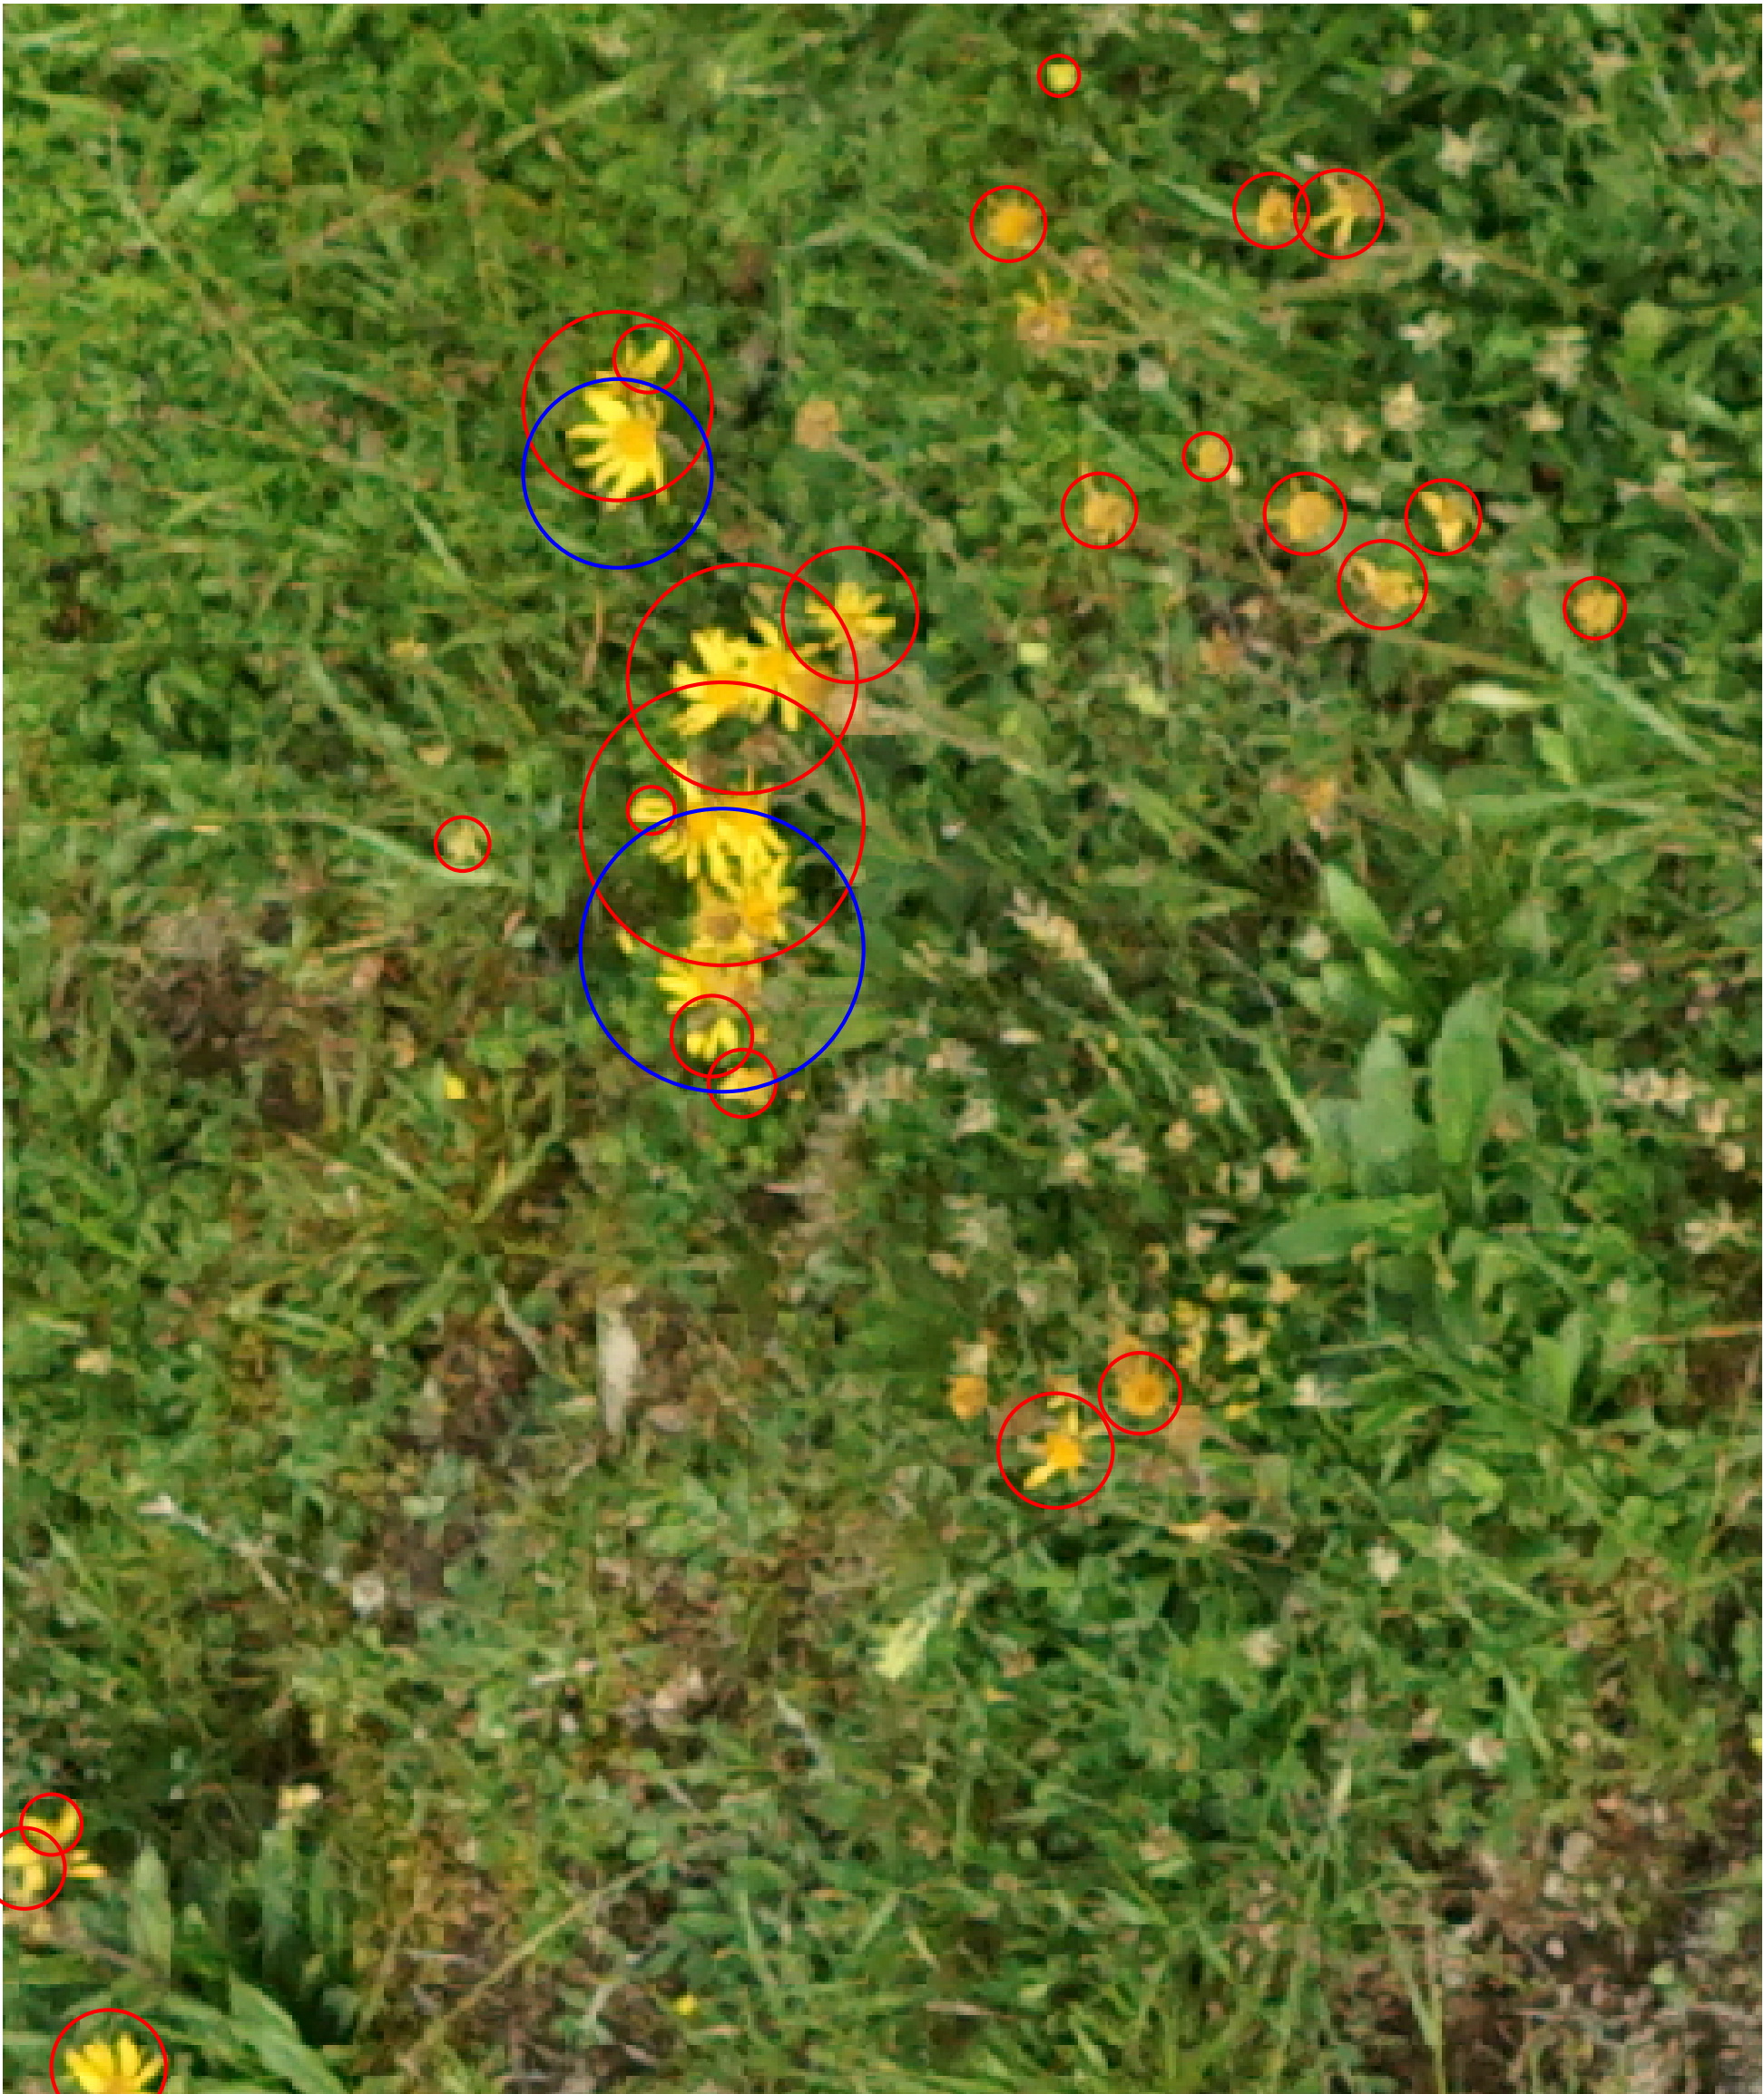
\includegraphics[width=0.4\textwidth,angle=0]{abb/ergebnisse/probleme/circles-adjust2}
 \caption{Kreise nur bei großen CC hinzugefügt (blau)}
\label{fig:Kreis-blau2}
\end{figure}

Kritische Reflektion, ob das so erfolgreich war...

\subsubsection{Problem: Blume wird durch Schatten gestückelt}

Idee: Smoothing edges vor segmentation um trennungen der Blüten rückgängig zu machen


Verbesserungsmöglichkeiten
Die eigenen Ergebnisse werden nicht über- oder unterbewertet

\subsubsection{Problem: Verwechslungspotential Arnica montana}

 schwer zu verhindern, aber durch andere faktoren identifikation -> GSM und Höhe der Pflanzen oder Bodensäure?

